\documentclass[dvipdfmx]{article}
\usepackage[dvipdfmx]{graphicx}
\usepackage{amsmath, amssymb}
\usepackage{mathtools}
\usepackage{here}

\begin{document}
\title{Weekly Report}
\author{Riku Gondow}
\maketitle
\section{Progress}
\begin{itemize}
    \item Train and evaluate LSTM using 30-subjects dataset
    \item Train and evaluate ResNet101 using 30-subjects dataset
\end{itemize}

\section{LSTM-CNN Ensemble Method\cite{lstm}}
When I evaluated with data from 30 subjects, the accuracy did not improve much, so I evaluated with data from 5 subjects.

As a result, the method that worked well for ECG did not work well for the radar signal.

\subsection{Evaluation of LSTM}

\begin{figure}[H]
\begin{center}
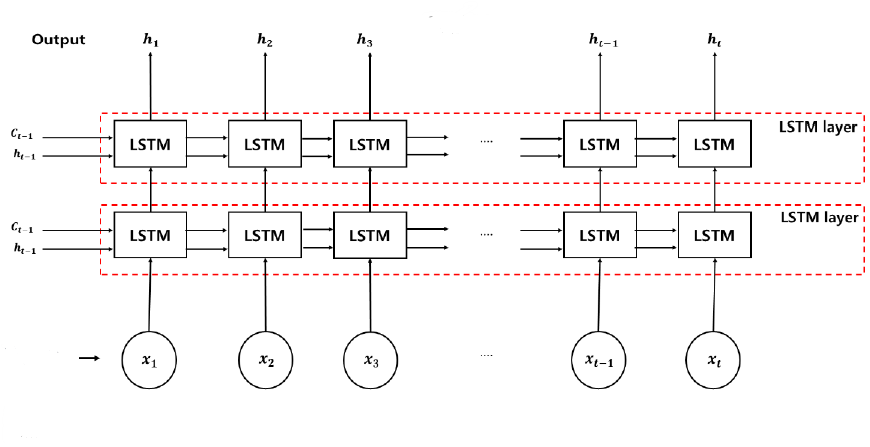
\includegraphics[width=\linewidth]{./img/LSTM.png}
\end{center}
\caption{The structure of Two-Layered LSTM}
\end{figure}

The radar signal recorded at 2000 Hz was down-sampled to 250 Hz, the window size was set to 4 s, and the overlap was set to 1.4 s.

\begin{table}[H]
\caption{Hyper parameter and Accuracy}
\centering
\begin{tabular}{cc}
\hline
Number of classes & 5 \\
Number of epochs & 300 \\
Learning rate & 0.01\\
Hidden size & 100 \\
Number of layers & 2 \\
Accuracy & 31.6\% - 69.6\% \\
\hline
\end{tabular}
\end{table}

\subsection{Evaluation of ResNet101}

\begin{figure}[H]
\begin{center}
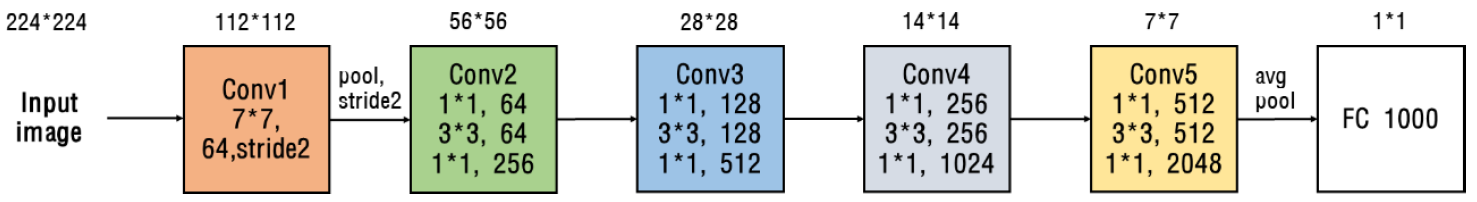
\includegraphics[width=\linewidth]{./img/ResNet101.png}
\end{center}
\caption{The structure of ResNet101}
\end{figure}

I used the pre-trained ResNet101 and trained with spectrograms generated from radar signals.

When the radar heartbeat signal was used, the length corresponding to one beat of ECG did not show characteristics unique to each individual. Therefore, a window size corresponding to approximately 10 beats (not exact) was selected.

\begin{figure}[H]
\begin{center}
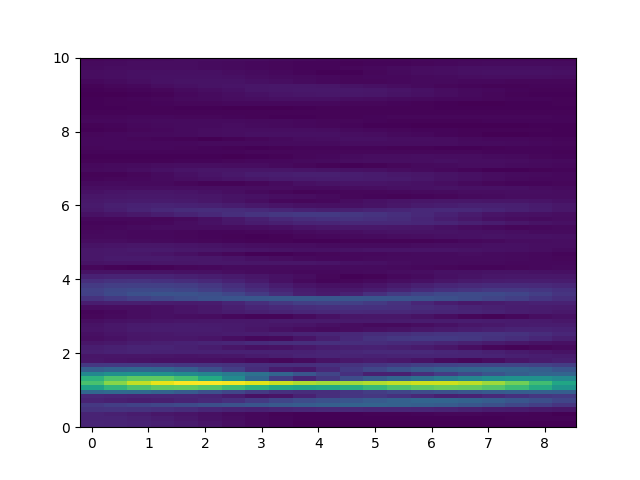
\includegraphics[width=\linewidth]{./img/stft_01_010.png}
\end{center}
\caption{Spectrogram of subject1 used for training. The horizontal and vertical axes represent time and frequency, respectively}
\end{figure}

\begin{table}[H]
    \caption{Hyper parameter and Accuracy}
    \centering
    \begin{tabular}{cc}
    \hline
    Number of classes & 5 \\
    Number of epochs & 30 \\
    Learning rate & 0.01 \\
    Accuracy & 21.9\% \\
    \hline
    \end{tabular}
\end{table}


\section{Next Plan}
\begin{itemize}
    \item Consider the reasons why it didn't work
    \item Survey the radar-based method and consider other methods
\end{itemize}

\begin{thebibliography}{99}
    \bibitem{lstm} Lee, Jin-A., and Keun-Chang Kwak. "Personal Identification Using an Ensemble Approach of 1D-LSTM and 2D-CNN with Electrocardiogram Signals." Applied Sciences 12.5 2022: 2692.
\end{thebibliography}
\end{document}